\documentclass[11pt]{beamer}
\usetheme{Rochester}
\usecolortheme{seagull}
\usepackage[utf8]{inputenc}
\usepackage[german]{babel}
\usepackage[T1]{fontenc}
\usepackage{amsmath}
\usepackage{amsfonts}
\usepackage{amssymb}
\usepackage{textpos}

% add logo to the sections
\addtobeamertemplate{frametitle}{}{%
\begin{textblock*}{100mm}(.6\textwidth,-1.2cm)

\includegraphics[width=0.5\linewidth]{./logo_inf_fak.png}
\end{textblock*}}


\setbeamertemplate{footline}[frame number]

\author{Größler, Hofmann, Zettwitz, Sopauschke, Sturm, Solovjova}
\title{A visualization technique for \\  hierarchical edge bundles}
\date{14.Januar 2016} 
%\setbeamercovered{transparent}  
%\subject{}


\begin{document}

\begin{frame}
\titlepage
\end{frame}

\begin{frame}
\frametitle{Inhalt} 
\tableofcontents
\end{frame}


\section{Ziel des Projekts}
\begin{frame}
\frametitle{Ziel des Projekts}
\begin{itemize} 
\item hierarchische Graphdaten (Baum)
\item Radiales Layout der Graphdaten
\item Bündelung der Graphdaten(Pfade) durch B-Splines
\item Echtzeit/interaktive Visulaisierung
\end{itemize}
\end{frame}

\section{Verwendetes Paper}
\begin{frame}[allowframebreaks]
\frametitle{Verwendetes Paper}
\begin{itemize} 
\item Hierarchical Edge Bundles: \\
Visualization of Adjacency Relations in Hierarchical Data
\item Autor: Danny Holton
\item Jahr: 2006
\end{itemize}
\end{frame}

\subsection{Graphenstrukturen}
\begin{frame}
\frametitle{Graphenstrukturen}
\begin{itemize}
\item Rooted tree
\item radial tree
\item balloon tree
\item tree map
\begin{textblock*}{150mm}(4cm,-2cm)
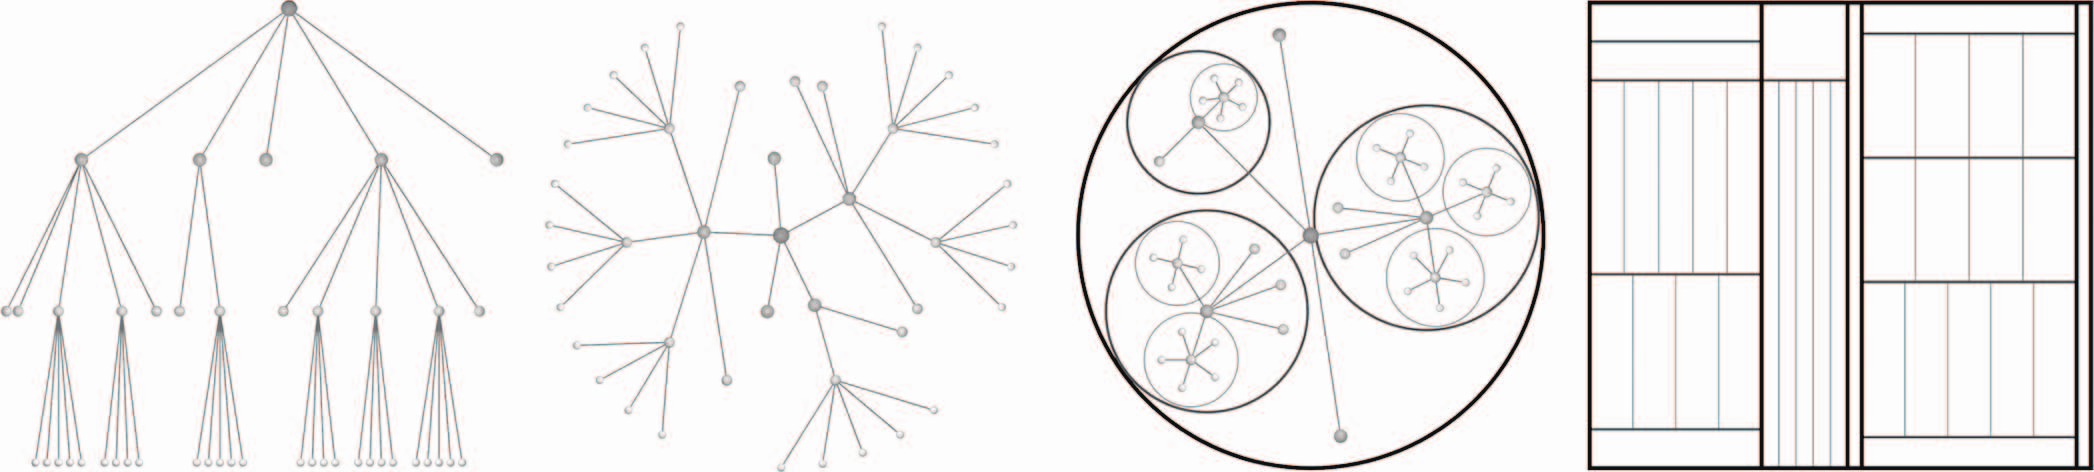
\includegraphics[width=0.5\linewidth]{./TreeTypes.png}
\end{textblock*}
\end{itemize}

\end{frame}

\subsection{Radial Layout}
\begin{frame}
\frametitle{Radial Layout}

\begin{itemize}
\item Bessere Nutzung der Fläche durch radiales Layout
\item Level bilden "Kreisringe", Wurzel ist Mittelpunkt
\end{itemize}

\section{Compound Graph}
\begin{frame}[allowframebreaks]
\frametitle{Compound Graph}

Compound Graph Bestandteile:
\begin{itemize} 
\item Wurzel
\item Knoten (Eltern, Kind)                                                                                                                       
\item Level, Link(Ziel), Position(x,y)
\item Anzahl an Kindern auf allen Leveln
\end{itemize}

\framebreak
\begin{itemize} 
\item Pfad nur von Blatt zu Blatt
\item Shortest path: von beiden Endpunkten aufsteigen, \\ bis gemeinsamer Knoten erreicht wurde
\item Speichere jeden besuchten Knoten (später für Splines benötigt)
\item Zufallsgenerierung: \#Level, \#Knoten, \#avg. Kinder, \#Links
\end{itemize}

%Übersichtsbild der Klassen einfügen

\end{frame}


\section{Radial Layout}
\begin{frame}
\frametitle{Radial Layout}

\begin{itemize}
\item Bessere Nutzung der Fläche durch radiales Layout
\item Level bilden "Kreisringe", Wurzel ist Mittelpunkt
\item Anzahl aller Kinder bestimmt konzentrisch Position auf Ring 
\\ und bildet Sektor (alle weiteren Kinder innerhalb)
\end{itemize}

%Michis Formel einfügen (sin...cos...)
%Bild einfügen

\end{frame}


\section{Splines}
\begin{frame}
\frametitle{Splines}

\begin{itemize}
\item dummy splines allgemein
\end{itemize}

\end{frame}



\subsection{B-Splines}
\begin{frame}
\frametitle{B-Splines}

\begin{itemize}
\item dummy
\end{itemize}

\end{frame}



\section{Technnisches System}
\begin{frame}
\frametitle{Technisches System}

\begin{itemize}
\item Cross-platform: gestestet unter Windows 8, Ubuntu 14.04
\item Cmake als build-tool
\item OpenGL(GLUT, GLEW) als plattformunabhängige  
\\ Anbindung an Grafikkarte -> schnell(GPU beschleunigt) 
\item Erzeugung des Graphen auf CPU
\item Berechnung der Splines, Rendering auf GPU (Shader)
\end{itemize}

\end{frame}



\section{Demo}
\begin{frame}
\frametitle{Demo}

Es folgt eine kurze Demonstration unserer Ergebnisse

\end{frame}


\section{Nutzen und Erweiterung}
\begin{frame}
\frametitle{Nutzen und Erweiterung}

\begin{itemize}
\item Datenexploration...
\item Erweiterung: allgemeine Graphen (durch betweeness centrality)
\end{itemize}

\end{frame}


\end{document}